% !TEX root = main.tex
\section{Numerical examples}\label{sec:numerical}
\subsection{A Linear mixed effects model}
\subsubsection{The model}
We consider, in this section, a linear mixed effects model \citep{lavielle2014Mixed}.
We denote by $y = (y_i \in \rset^{n_i}, i \in \inter)$ the observations where for all $i \in \inter$:
\begin{equation}
y_i = A_i\theta + B_iz_i + \epsilon_i \quad.
\end{equation}
$A_i \in \mathbb{R}^{n_i \times p}$ and $B_i \in \mathbb{R}^{n_i \times m}$ are design matrices, $\theta \in \mathbb{R}^{p}$ is a vector of parameters, $z_i \in \mathbb{R}^{m}$ are the latent data (i.e. the random effects in the context of mixed effects models) which are assumed to be distributed according to a multivariate Gaussian distribution $\mathcal{N}(0,\Omega)$ where $\Omega \in \mathbb{R}^{m \times m}$. We also assume that the residual errors $\epsilon_i \in \mathbb{R}^{n_i}$ are distributed according to $\mathcal{N}(0,\Sigma)$, where $\Sigma \in \mathbb{R}^{n_i \times n_i}$, and that the sequences of variables $(z_i, i \in \inter)$ and $(\epsilon_i, i \in \inter)$ are i.i.d. and mutually independent. The covariance matrices $\Omega$ and $\Sigma$ are assumed to be known. For all $i \in \inter$, the conditional distribution of the observations given the latent variables $y_i|z_i$ and of the latent variables given the observations $z_i|y_i$ are respectively given by:
\begin{align}
& y_i|z_i \sim \mathcal{N}(A_i\theta + B_iz_i,\Sigma),\\
& z_i|y_i \sim \mathcal{N}(\mu_i, \Gamma_i).
\end{align}
where:
\begin{align}\label{posteriormean}
&\Gamma_i =  (B_i^\top \Sigma^{-1} B_i + \Omega^{-1})^{-1},\\
&\mu_i = \Gamma_i B_i^\top\Sigma^{-1} (y_i - A_i\theta).
\end{align}
% Assumption M\ref{twicediff}\ref{post} is thus verified since $|\nabla^2\log p_i(z_i,\theta)| = \Gamma_i^{-1}$. The negated incomplete log likelihood $\loglike(\theta)$ is given by:
% \begin{equation}\label{incompletelog}
% \loglike(\theta) \propto \sum_{i=1}^{N}{(y_i - A_i\beta)^\top \left(B_i\Omega B_i^\top+\Sigma\right)^{-1} (y_i - A_i\beta)}
% \end{equation}
% Assumption M\ref{bounded} is trivially verified. The complete log likelihood $\log f(z,\theta)$ is given by:
% \begin{equation}\label{completelog}
% \log f(z,\theta) \propto -\sum_{i=1}^{N}{(y_i-A_i\beta - B_iz_i)^\top\Sigma^{-1}(y_i-A_i\beta - B_iz_i)}
% \end{equation}
% Here $\Theta \triangleq \mathbb{R}^{d}$ (M\ref{convex} verified) and for all $i \in \inter$, $\tilde{S}_i(z_i) \triangleq z_i$. Since:
% \begin{alignat*}{2}
% & \nabla f_i(z_i,\theta) = && A_i^\top \Sigma^{-1}(y_i - A_i\hat{\beta}- B_iz_i)f_i(z_i,\theta)\\
% & \nabla^2 f_i(z_i,\theta) = && -A_i^\top A_i \Sigma^{-1}f_i(z_i,\theta) \\
% & &&+ A_i^\top \Sigma^{-1}(y_i - A_i\hat{\beta}- B_iz_i)\nabla f_i(z_i,\theta)
% \end{alignat*}
% we verify assumptions M\ref{twicediff}\ref{complete} and M\ref{twicediff}\ref{smoothness}.
This model belongs to the curved exponential family introduced in section \ref{sssec:expo} where for all $i \in \inter$:
\begin{align}\label{statmem}
& \tilde{S}_i(z_i) \triangleq z_i \quad \textrm{and} \quad \bar{s}_i(\theta) =  \Gamma_i B_i^\top\Sigma^{-1} (y_i - A_i\theta)\\
& \psi_i(\theta) \triangleq  (y_i - A_i\theta)^\top\Sigma^{-1}(y_i - A_i\theta)\\
& \phi_i(\theta) \triangleq B^\top \Sigma^{-1} (y_i - A_i\theta)
\end{align}
Maximising $L(s,\theta)$, defined in \eqref{curvedL}, with respect to $\theta$ yields the following maximisation function for all $s=(s_i \in \mathbb{R}^{m}, i \in \inter)$:
\begin{equation*}
\hat{\theta}(s) \triangleq \left(\sum_{i=1}^{N}{A_i^\top \Sigma^{-1}A_i}\right)^{-1}\sum_{i=1}^{N}{A_i^\top \Sigma^{-1}(y_i - B_i s_i)}.
\end{equation*}
Thus, the $k-th$ update of the MBEM algorithm consists in sampling a subset of indices $I_k$ and computing $\theta^k = \hat{\theta}(s^k)$ where:
\begin{align*}
  s_i^k &=
  \begin{cases}
   \bar{s}_i(\theta^{k-1})        & \text{if } i \in I_k. \\
   s_i^{k-1}         & \text{otherwise}.
  \end{cases}
\end{align*}
\subsubsection{Simulation and runs}
We generate a synthetic dataset, with $d = 2$, $\theta: (\theta_1:4,\theta_2:9)$, $N=10000$ and for all $i \in \inter$, $n_i = 10$ observations per individual and random design matrices $(A_i, i \in \inter)$ and $(B_i, i \in \inter)$. Two runs of the MBEM are executed starting from different initial values ($(\theta_1^0:1,\theta_2^0:5)$ and $(\theta_1^0:3,\theta_2^0:7)$) to study the convergence behaviour of these algorithms depending on the initialisation.
Figure \ref{iem_glm} shows the convergence of the vector of parameter estimates $(\theta_1^k,\theta_2^k)_{k=0}^{K}$ over passes of the EM algorithm, the MBEM algorithm where half of the data is considered at each iteration and the Incremental EM algorithm (i.e. a single data point is considered at each iteration). The speed of convergence is a monotone function of the batch size in this case, the smaller the batch the faster the convergence.
\begin{figure}
\begin{center}
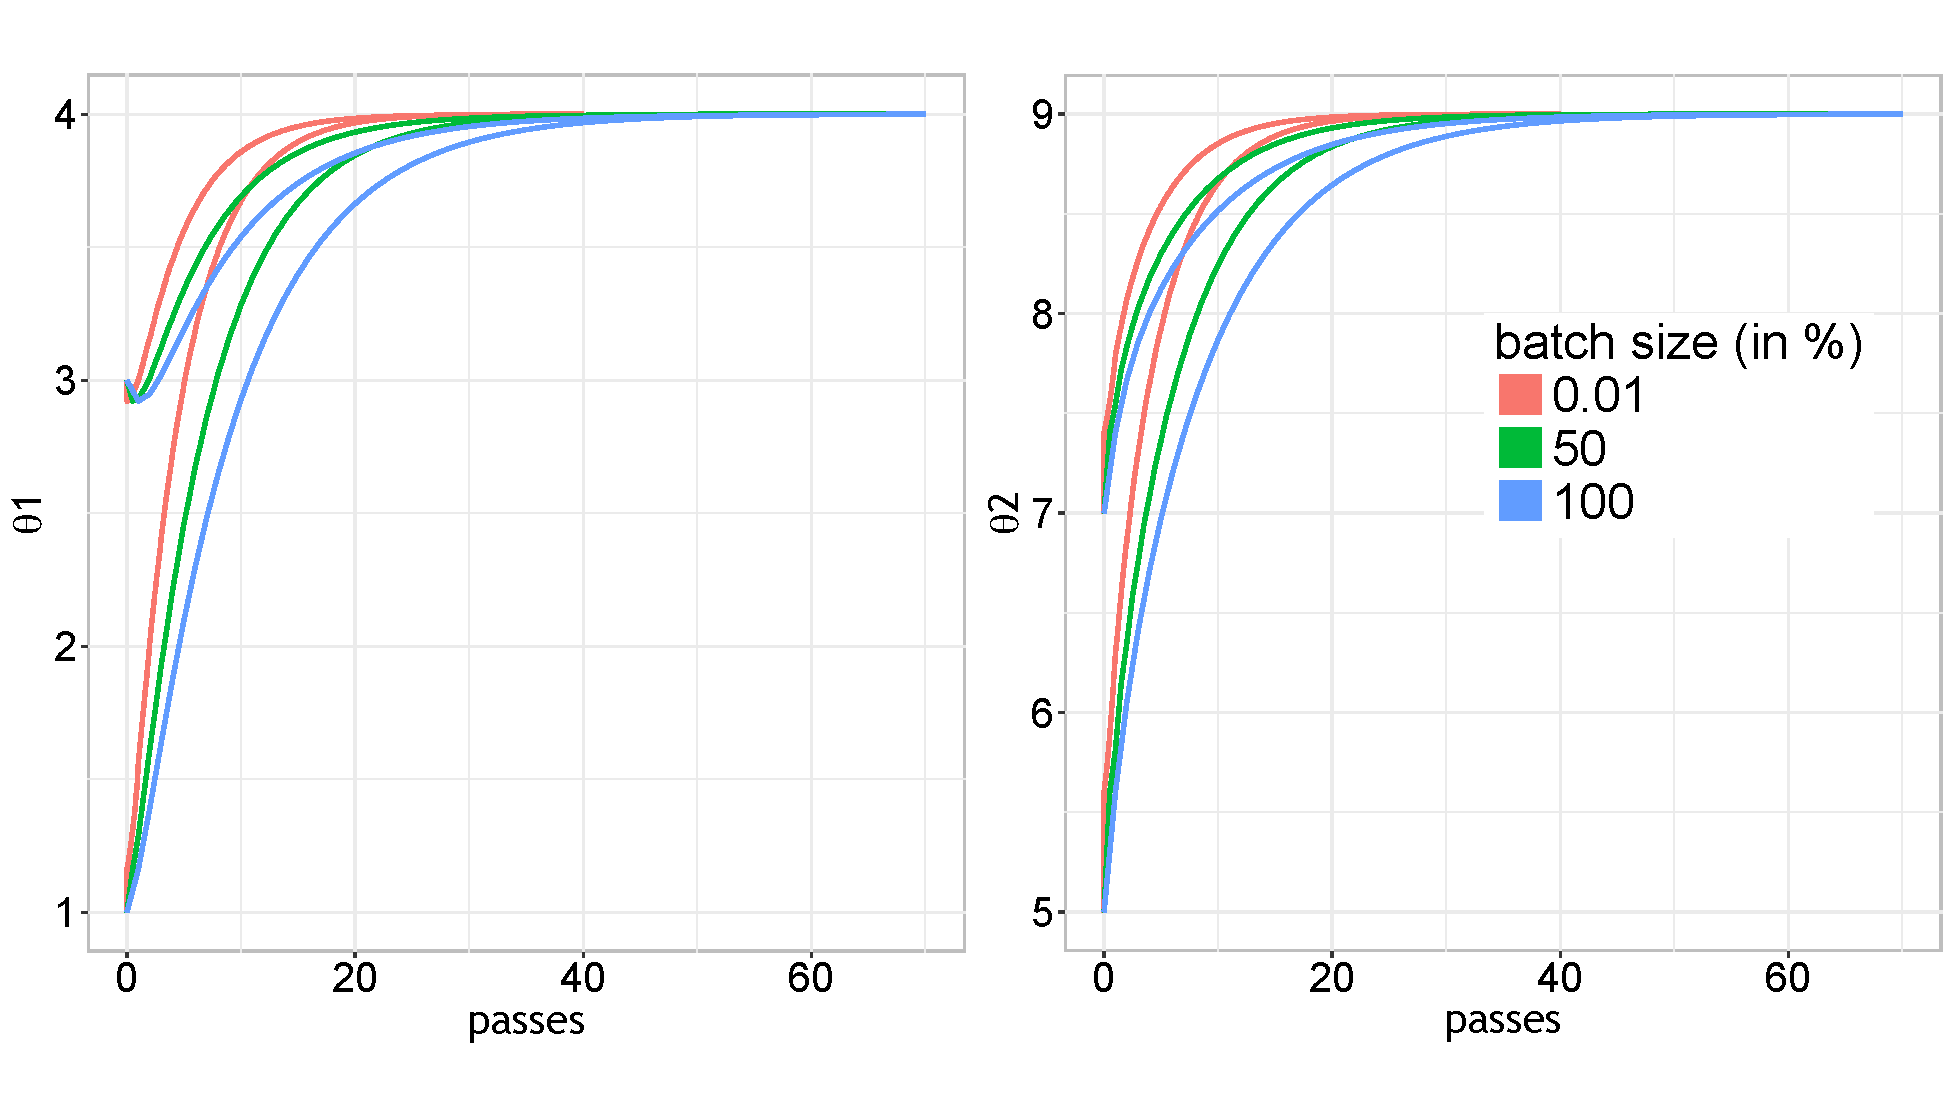
\includegraphics[scale = 0.35]{pics/iems.pdf}
\caption{Convergence of the vector of parameter estimates $\theta^k$ function of passes over the data.}
\label{iem_glm}
\end{center}
\end{figure}


